\documentclass[pdf, aspectratio=169]{beamer}
\usepackage[]{hyperref,graphicx,siunitx,lmodern,booktabs,tikz,caption}
\usepackage{pdfpc-commands}


\usepackage[mode=buildnew]{standalone}
\mode<presentation>{\usetheme{Astro}}

\graphicspath{ {../Images/} }

\sisetup{per-mode=symbol}
\usetikzlibrary{calc,angles,quotes}

%preamble
\title{Connecting the Dots}
\date{August 29, 2018}
\author{Jed Rembold}

\begin{document}
\renewcommand*{\theenumi}{\Alph{enumi}}

\begin{frame}{Announcements}
	\begin{itemize}
	  \item We'll be working through Chapter 2 the next several classes
	  \item If you didn't complete HW1, it isn't too late to still do for most of the credit!
	  \item HW2 will be available today after class. Due 10am on Friday.
	  \item Tutoring is starting up on Sunday
		  \begin{itemize}
		  	\item Sun-Thur 7:30-9:30pm in the Physics hearth
		  \end{itemize}
	  \item Polling: \url{rembold-class.ddns.net}
	\end{itemize}
\end{frame}

\begin{frame}{Astronomy Picture of the Day}
  \begin{figure}[h!]
	\centering
	\includegraphics[width=.7\textwidth]{APOD_SunEclipse.jpg}
  \end{figure}
\end{frame}

\begin{frame}{Review Question}
	A light-year is approximately:
  \begin{enumerate}
	\item \SI{8}{\minute}
	\item \SI{365}{\day}
	\item \SI{5}{AU}
	\item \alert<2>{\SI{9.45E15}{\meter}}
  \end{enumerate}
  \vspace{1cm}
  \emph{Hint: the speed of light is \SI{3e8}{\meter\per\second}.}
\end{frame}

\begin{frame}{A View from Earth}
  \begin{figure}[h!]
	\centering
	\includegraphics<1>[width=.7\textwidth]{ch2_Sky.png}
	\includegraphics<2>[width=.7\textwidth]{ch2_Sky_w_Lines.png}
	\includegraphics<3>[width=.7\textwidth]{ch2_Sky_w_Pics.png}
  \end{figure}
\end{frame}

\begin{frame}{Constellation Details}
  \begin{itemize}
	\item Stars may only \emph{appear} to be next to one another
	  \begin{itemize}
		\item In reality they may be (and likely are) separated by light-years and parsecs of space
	  \end{itemize}
	\item Stars are so far away that we lose depth perception
	  \begin{itemize}
		\item Think far away headlights at night
	  \end{itemize}
	\item Our eyes could not tell the difference between space as we know it and us living in a huge dark bubble with holes in it to let in light
	\item Thus we commonly refer to the \alert{Celestial Sphere}
  \end{itemize}
\end{frame}

\begin{frame}{The Celestial Sphere}
  \begin{itemize}
	\item Aligned with Earth's sphere
	  \begin{itemize}
		\item North and South poles align
		\item Equator Aligns
	  \end{itemize}
	\item Equator does \alert{not} align with the Solar System's disk, because Earth is tilted
	  \begin{itemize}
		\item The \alert{ecliptic} is the path the Sun (and planets) follow through our sky.
	  \end{itemize}
	\item Like the Earth, positions are denoted with latitude and longitude!
	  \begin{itemize}
		\item Commonly called Declination and Right Ascension, respectively.
	  \end{itemize}
  \end{itemize}
\end{frame}

\begin{frame}{Orientation and Vocabulary}
  \begin{figure}[h!]
	\centering
	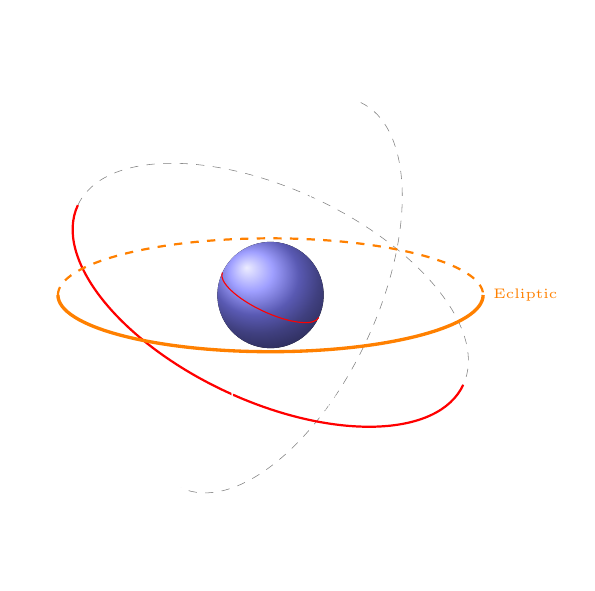
\begin{tikzpicture}[draw=white, every node/.style={white,font=\tiny},scale=.9, rotate=-25]
		\draw (0,0) circle(3);
		\draw[help lines, dashed] (0,3) arc (90:-90:1.5cm and 3cm);
		\draw (0,3) arc (90:270:1.5cm and 3cm);
		\draw[help lines, dashed] (-3,0) arc (180:0:3cm and 1.5cm);
		\draw[red,thick] (-3,0) arc (180:360:3cm and 1.5cm) node[pos=0.75,above,align=center,xshift=-3mm] {Celestial\\Equator} ;

		\draw (0,-.8) node[below,align=center] {Earth\\South\\Pole} -- (0,.8) node[above,align=center] {Earth\\North\\Pole};
		\fill[ball color=blue!50] (0,0) circle (0.75cm);
		\draw[red] (-.75,0) arc (180:360:.75cm and .25cm);

		\draw (0,3) -- (0,3.2) node[above,align=center] {Celestial\\North\\Pole};
		\draw (0,-3) -- (0,-3.2) node[below,align=center] {Celestial\\South\\Pole};
		\pause
		\draw[orange, rotate=25, very thick] (-3,0) arc (180:360:3cm and .8cm);
		\draw[orange, rotate=25, dashed,thick] (-3,0) arc (180:0:3cm and .8cm) node[right,orange] {Ecliptic};
		\onslide<1->
	  \end{tikzpicture}
  \end{figure}
\end{frame}

\begin{frame}{From Our Perspective}
  \begin{figure}[h!]
	\centering
	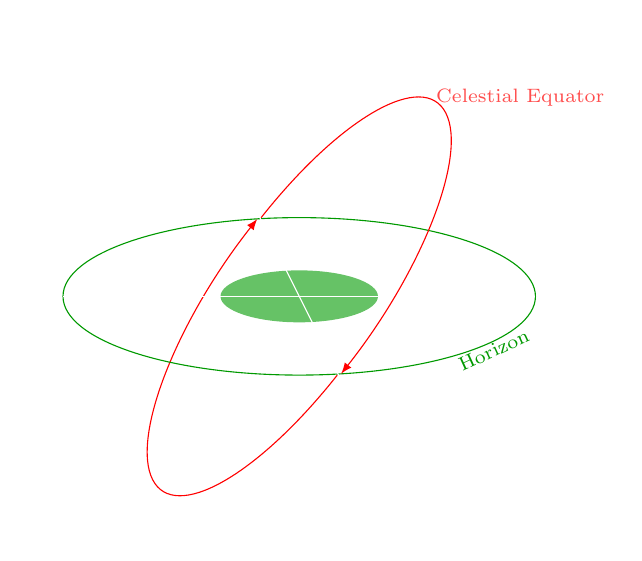
\begin{tikzpicture}[draw=white, every node/.style={white, font=\scriptsize}]
	  \draw (0,0) circle(3);
	  \draw[red,latex-,yscale=-1,rotate=-235] (-.5,1) arc (100:-80:3cm and 1cm);
	  \fill[black!40!green, opacity=0.6] (0,0) ellipse (1cm and 0.33cm);
	  \draw[black!40!green] (-3,0) arc (180:540:3cm and 1cm) node[black!40!green, pos=.4,sloped,yshift=-3pt] {Horizon};
	  \draw (-3,0) node[left] {N} -- (3,0) node[right] {S};
	  \draw (-.5,1.0) node[above left] {E} -- (.5,-1) node[below right] {W};
	  \draw[red,latex-,yscale=-1,rotate=-55] (-.5,1) arc (100:-80:3cm and 1cm) node[pos=.6, red!70, right] {Celestial Equator};
	  \begin{scope}[rotate=45]
		\draw[fill=white](0,3) circle(0.75mm) node[below right,align=center] {Celestial\\North}-- (0,4);
		\draw[-latex] (0.1,3.4) arc (70:-250:.30cm and .10cm);
		\draw[fill=white] (0,-3) circle(0.75mm) node[above left, align=center] {Celestial\\South} -- (0,-4);
	  \end{scope}
	  \fill[white] (0,3) circle(.75mm) node[above] {Zenith};
	  \draw (.6,1.6) -- (1,2) node[xshift=2pt,yshift=2pt] {$\star$};
	  \draw (.1,1.3) -- (.5,1.7) node[xshift=2pt,yshift=2pt] {$\star$};
	\end{tikzpicture}
  \end{figure}
\end{frame}

\begin{frame}{How Things Move: As we see it}
  \begin{itemize}
	\item Furthest away: Stars
	  \begin{itemize}
		\item Move along parallel to the Celestial equator
	  \end{itemize}
	\item Closing in: Solar System Objects
	  \begin{itemize}
		\item Move along parallel (and near to) the ecliptic
	  \end{itemize}
	\item Other Objects: Milky Way
	  \begin{itemize}
		\item Galactic plane does not line up with Solar System
		\item We see the Milky Way oriented in the sky at yet another angle ($\approx$\SI{63}{\degree} from the Celestial equator)
		\item Motion follow that of the stars, parallel to the Celestial equator
	  \end{itemize}
  \end{itemize}
\end{frame}

\begin{frame}{Making Measurements}
  With everything on a sphere, how do we make measurements?\pause
  \begin{itemize}
	\item With angles! (commonly called \alert{angular distance})
	  \begin{itemize}
		\item Using your outstretched arm:
		  \begin{itemize}
			\item Pinky width = \SI{1}{\degree}
			\item 3 middle finger width = \SI{5}{\degree}
			\item Fist width = \SI{10}{\degree}
			\item Spread hand width = \SIrange{20}{25}{\degree}
		  \end{itemize}
		\item We often need to break degrees into smaller increments:
		  \begin{itemize}
			\item 60 arc-minute = \SI{60}{\arcminute} = \SI{1}{\degree}
			\item 60 arc-second = \SI{60}{\arcsecond} = \SI{1}{\arcminute}
		  \end{itemize}
		\item Longitude angles sometimes given in hours
		  \begin{itemize}
			\item Earth rotates \SI{360}{\degree} in \SI{24}{\hour}
			\item Thus \SI{1}{\hour} $\approx$ \SI{15}{\degree}
		  \end{itemize}
		\item Angular size related to physical size by the distance away (via trig)
	  \end{itemize}
  \end{itemize}
\end{frame}

\begin{frame}{Arc-Time}
	\begin{example}
		Convert \ang{39;47;32} to its decimal representation.
		\pause
		\begin{align*}
			\ang{;;32} \times \frac{\ang{;1;}}{\ang{;;60}} &= \ang{;0.533;}\\
			\ang{;47;} + \ang{;0.533;} &= \ang{;47.533;} \\
			\ang{;47.533;} \times \frac{\ang{1}}{\ang{;60;}} &= \ang{0.7922}\\
			\ang{39} + \ang{.7922} &= \ang{39.7922}
		\end{align*}
	\end{example}
\end{frame}

\begin{frame}{Angular $\rightarrow$ Physical Size}
	As long as the angular sizes are small, we can relate angular size and physical size via:
	\[\frac{\text{Angular Size}}{\SI{360}{\degree}} = \frac{\text{Physical Size}}{2\pi(\text{Distance Away})}\]
	\begin{example}
		Given that, how far away is the back of the room from the circle on the front board?
	\end{example}
\end{frame}

\begin{frame}{Clarification}
  \begin{alertblock}{Don't Get Confused!}
	Angular distances are the same using either the Celestial coordinate system or the local coordinate system
  \end{alertblock}
  \begin{itemize}
	\item Celestial System:
	  \begin{itemize}
		\item Celestial Latitude (Declination)
		\item Celestial Longitude (Right Ascension)
		\item Think in terms of the globe
	  \end{itemize}
	\item Local System
	  \begin{itemize}
		\item Direction you are looking (Azimuth)
		  \begin{itemize}
			\item Determined by compass usually
		  \end{itemize}
		\item Angular distance above horizon (Altitude)
		  \begin{itemize}
			\item Can determine with a sextant or estimate with your hands
		  \end{itemize}
	  \end{itemize}
  \end{itemize}
\end{frame}

\begin{frame}{Understanding Check}
  Supposed I asked you for the angular diameter of a circle drawn at the front of the room. The students in the front row would measure an angular distance that is \underline{\hspace{2cm}} the students in the back row.
  \begin{enumerate}
	\item \alert<2>{larger than}
	\item smaller than
	\item equal to
	\item opposite to
  \end{enumerate}
\end{frame}

\begin{frame}{Celestial Sphere Demonstrations}
  \begin{example}
	\begin{itemize}
	  \item How long is the sun up today here on the 45th parallel?
	  \item How long is the sun up today up in Alaska on the 65th parallel?
	  \item How high will the sun rise in the sky for us on December 10th?
	  \item What time will Orion rise on October 31?
	  \item What altitude and azimuth will Vega have at midnight tonight?
	\end{itemize}
  \end{example}
\end{frame}


\end{document}
